\section{Prediction Meta Modeling}

This section describes how a multilayer perceptron can be used to aggregate scalar prediction scores.
We will first go through the modeling phase, where each method and network is trained.
Second, we will show how these trained models are used to personalized method aggregation.


\subsection{Modeling Phase}

We shall now use a multilayer perceptron to create a personalized aggregation method.
Before we can start blending predictions, we have to create the individualized neural networks.
This requires training the user modeling methods, and the network itself.
We also have to test the resulting models.
Naturally, this makes partitioning the data a bit of a challenge, as we have two successive levels of user models to train.
We basically need three types of datasets: 

\begin{enumerate*}
  \item Training sets to create the standard modeling methods.
  \item Training sets to create the personalized neural networks.
  \item A testing set to test our final system.
\end{enumerate*}

Constructing these subsets of the available data is a common task in ensemble learning.
We shall use an approach known as  \emph{bootstrap aggregating} (\emph{bagging}),
introduced by \cite{Breiman1996}.
Originally, bagging is an ensemble learning classification methods, where multiple classifiers are 
trained by uniformly sampling a subset of the available training data. 
Each model is then trained on one of these subsets, and the models are aggregated by averaging their individual predictions.

Formally, given a training set $D$ with $n$ items, bagging creates $m$ new training sets of size $n' \leq n$ by sampling
items from $D$ uniformly and with replacement. 
In statistics, these types of samples are called \emph{bootstrap samples}.
If $n'$ is comparable in size to $n$, there will be some items
that are repeated in the new training sets.

Bagging suits our needs perfectly, for a few reasons: First, the method helps create disjoint predictors, 
since each predictor is only trained (or specialized for) a subset of the available data.
Second, it allows us to easily train the underlying modeling methods without any complex partitioning of the data.
Our partitioning strategy is now clear:

\begin{enumerate*}
  \item Split the entire dataset into a training and testing set.
  \item Train modeling methods through bootstrap aggregation of the training set.
  \item Train personalized network from each user's ratings from the training set.
  \item Test the resulting personalized aggregation model with the testing set.
\end{enumerate*}

Each modeling method is trained in ways specific to their implementation. 
Model-based approaches create pre-built strutures and provide offline training,
while heuristic methods simply store the data for future computation.
Either way, it is up to each modeling method what it does with the supplied training data.

Training the neural networks for each user is done through the backpropagation algorithm:
Each user has a set of known ratings that serve as training examples.
For each of these examples, the inputs are the predictions made by the modeling methods.
The desired output is the actual rating given by the user.
This requires that the underlying models are not all trained with the data point
specifying this exact rating, or that the methods disregard this datapoint during
the network training phase. Training our entire system then follows
the algorithm outlined in Listing \ref{code:training}.

\begin{figure*}
  \lstinputlisting[
    label=code:training,
    caption={The algorithm that performs training of a 
    user meta modeling system. Returns the trained methods and networks.
    This is an offline, pre-prediction training approach.}
  ]{../code/training}
\end{figure*}

The neural networks are model-based in that they are pre-computed before any predictions are made.
After training, each of these user-specific network models must be stored in our system.
Creating and saving an individual network for each user might seem like a daunting task,
but two characteristics makes this a perfectly valid approach:

\begin{itemize}
  \item 
    The training is performed offline, and can be done at any time.
    While the initial computational demand might be high,
    the training is performed before any predictions are made.
    Prediction performance is much more important than training performance
    in this scenario as it is during prediction we wish to quickly 
    present results to the user.
    It is also worth noting that each iteration in the two loops given in Listing \ref{code:training}
    are easily parallelizable, as each iteration is independent of the others.
  \item
    Storing a neural net is as simple as storing the trained connection weights.
    The overall network structure and activtion functions remain the same for each user.
    As demonstrated, an MP is a simple network with few nodes, resulting
    in a simple weight matrix that has to be stored for each user.
    The size of this matrix corresponds to the number of input methods
    and the number of hidden layers.
    This results in compact user meta models that can easily be stored.
\end{itemize}

There is also the question of when each network should be trained.
After all, as a user continues to explicitly rate more items,
or as more items arrive in the system, the output from underlying methods
will change, and the network must be updated to reflect this new reality.
This problem, called \emph{concept drift} is a common occurence in machine learning methods.
An optimal strategy would consider retraining the network after some preset number
of new ratings or items have been added. As the network emply offline training,
this strategy can work in the background, continously producing new or updated networks
while predictions rely on the previous generation of completed user models.


\subsection{Prediction Phase}

We now have a set of trained modeling method, and a set of personalized neural networks --- one for each user.
We now wish to use these models to perform predictions, that is, estimate unknown ratings between users and items.
The first step is to feed the item and user IDs into each of our standard modeling methods.
The output from these methods are the inputs to the current user's multilayer perceptron
(see Figure \ref{fig:metanetwork}).

\begin{figure}[t]
  \center
  \def\layersep{4cm}
  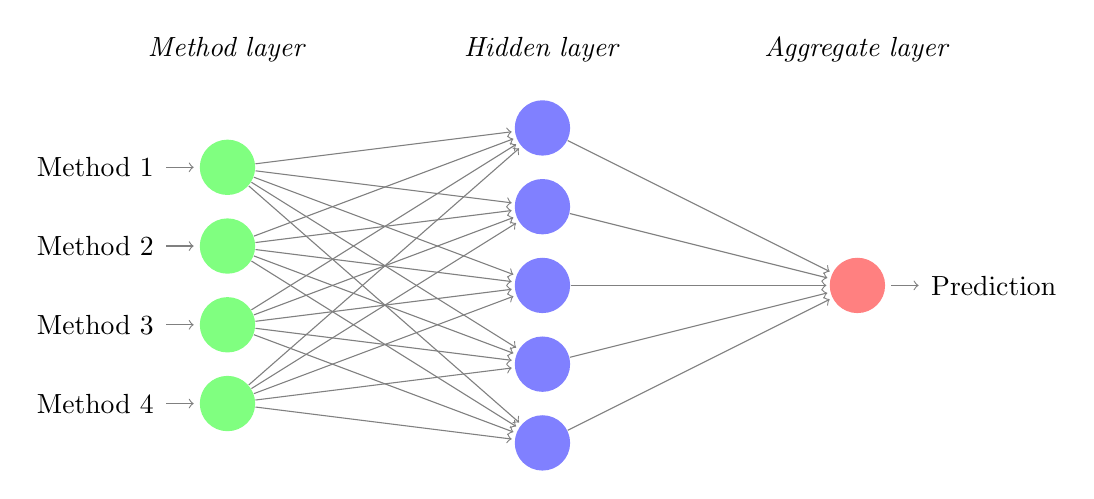
\begin{tikzpicture}[shorten >=1pt,->,draw=black!50, node distance=\layersep]

    \tikzstyle{every pin edge}=[<-,shorten <=2pt]
    \tikzstyle{neuron}=[circle,fill=black!25,minimum size=20pt,inner sep=0pt]
    \tikzstyle{input neuron}=[neuron, fill=green!50];
    \tikzstyle{output neuron}=[neuron, fill=red!50];
    \tikzstyle{hidden neuron}=[neuron, fill=blue!50];
    \tikzstyle{annot} = [text width=10em, text centered]

    % Draw the input layer nodes
    \foreach \name / \y in {1,...,4}
    % This is the same as writing \foreach \name / \y in {1/1,2/2,3/3,4/4}
        \node[input neuron, pin=left:Method \y] (I-\name) at (0,-\y) {};

    % Draw the hidden layer nodes
    \foreach \name / \y in {1,...,5}
        \path[yshift=0.5cm]
            node[hidden neuron] (H-\name) at (\layersep,-\y cm) {};

    % Draw the output layer node
    \node[output neuron,pin={[pin edge={->}]right:Prediction}, right of=H-3] (O) {};

    % Connect every node in the input layer with every node in the
    % hidden layer.
    \foreach \source in {1,...,4}
        \foreach \dest in {1,...,5}
            \path (I-\source) edge (H-\dest);

    % Connect every node in the hidden layer with the output layer
    \foreach \source in {1,...,5}
        \path (H-\source) edge (O);

    % Annotate the layers
    \node[annot,above of=H-1, node distance=1cm] (hl) {\emph{Hidden layer}};
    \node[annot,left of=hl] {\emph{Method layer}};
    \node[annot,right of=hl] {\emph{Aggregate layer}};
  \end{tikzpicture}

  \vspace{1em}
  \caption[User Meta Model Network]{
    The use of a multilayer perceptron for personalized model aggregation.
    This example takes the results from 4 different modeling methods,
    feeds them into a pretrained personalized neural net,
    and creates a combined prediction as output.}
  \label{fig:metanetwork}
\end{figure}


Translating the common terms used with ANNs, we have a \emph{method layer} corresponding to the input layer,
and an \emph{aggregation layer} corresponding to the output layer.
The number of nodes in the hidden layer is more a question for experimentation, as there are 
general rules on how many nodes this layer should have.
Regardless, this network topology allows us to combine multiple predictors into one personalized estimation.

Programatically, the prediction algorithm is as simple as Figure \ref{fig:metanetwork} suggests.
This algorithm is given in Listing \ref{code:prediction}, and follows the steps outlined above.
An important aspect is that step 1 in this algorithm is easily parallelizable. 
The application of each modeling method corresponds to the $\mathrm{map}$ step
explained in Section \ref{sec:usermetamodeling}.
Each modeling method can be run at the same time, as they remain independent of each other.
The network application in step 3 is then the $\mathrm{reduce}$ operation,
also from Section \ref{sec:usermetamodeling}.
As mentioned, expressing ourselves in terms of $\mathrm{map}$ and $\mathrm{reduce}$
will later guide our implementation of this algorithm.

\begin{figure*}
  \lstinputlisting[
    label=code:prediction,
    caption={The algorithm that performs prediction,
    i.e. estimating the unknown rating from user $u$ to item $i$.}
  ]{../code/prediction}
\end{figure*}





\section{Rank Meta Modeling}
\label{sec:methods:rank}

\subsection{Modeling Phase}

\subsection{Prediction Phase}

\section{Implementation}
